\section{Work Allocation(ps26g08)}

Working in a group has its advantages, but it also has drawbacks. The group has more man power and time, but the effectiveness of work allocation and other management skills must be achieved. Therefore, to use all the human resources as competent as possible. Although the developers have known about the specification of the project well, it is not so obvious how to implement the entirely approach to the project that is driven by some device which the members never have seen it before such as camera module, and the UAV. The following factor has been considered thoroughly before assigning task to any team members:

\begin{itemize}
\item	Availability of each member.

\item	The resource limitation
 
\item	The clarification of the task

\item   Time allowance for unexpected problems

\item	Each individual skills
\end{itemize}


\subsection{Planned Work Allocation}
 It is very essential that each member other coursework deadline and exams include in the consideration of work allocation. 
The engineer will work effectively if they got assigned  to their interest in the duty and that role clarified well. The work assign to each individual will be based on the posses sufficient skill and knowledge to perform the task. However, the team members must have flexibility in their time in order to support other team members when they have problems. Each task has been assigned a task leader and it will have the another member set to the same task in case the task leader has problems with the work they have done. In order to avoid work over run the time, the project has been set an earlier deadline so that if any unexpected problems happen, there are still a spare time to solve the problem. The specific skills that individuals want to mention are:

\begin{itemize}
\item Andy: Power, PCB, Control, MATLAB
\item Mitch: Image Processing, MATLAB, ASM, Report Writing
\item John: MATLAB, Image Processing, Control, Radio Transmission
\item Peak: Digital Control, Display, MATLAB, Information Theory
\item Michael: Programming, $\mu$Processors, Interfaces
\end{itemize}

Each member has variety of skills. Therefore the task has been located to each person according to this list.

The time line of the task is also important because some task for each individual depend on a completion of another task. This cause problems when one task got stuck and so the productiveness of the time management will be reduced. This can be solved by assigning another task that is not dependant on the other tasks. 

A Resource limitation is one of the factor that limited the group member to do tasks. This is because the customer provide only a single UAV and also only one camera has been purchased, so only one person can work on this device at a time. We solved this problem by having a laboratory space that the UAV will be placed their all the time so any of the team member can access it. To mange the limited resource, the only time that the individual access the UAV is when he wants to test the system. 

To clarify the tasks so the individuals can understand and also to ensure that all the tasks have been assigned to at least one member of the group is essential. 
The real development of this project will analyse the requirement from the start of how the project could be ensemble. The project will be a bottom-up design. It will start from each individual completion of a small task and then integrate them into a successful complete project. 
Figure\ref{task allocation} shows a diagram of task allocation to each member of the group. 
The task allocation based on the task locate on the block diagram in figure\ref{fig:block1}.
The blue box between members are the task shared between the members on it's side. 
If the blue box stand on its own it means only one person is assigned to that task.
This task allocation came up when we have meetings.
It has all the requirements to implement the final project.

\begin{figure}[H]
\begin{center}
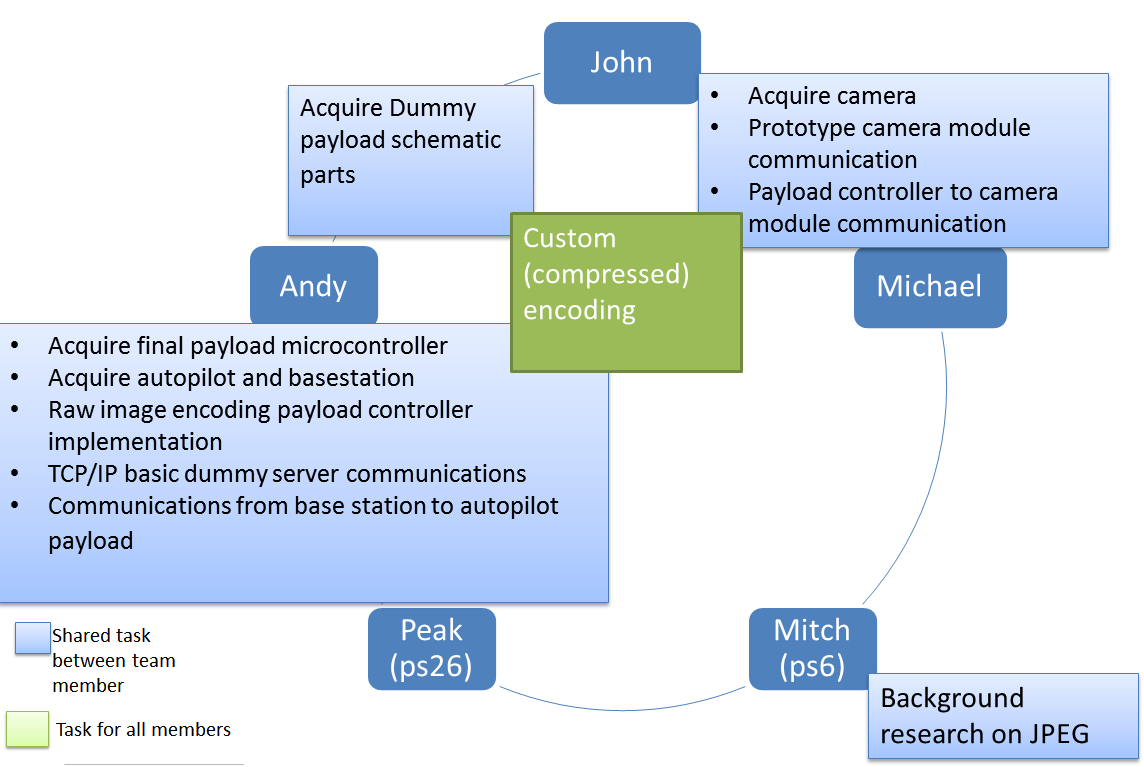
\includegraphics[width=1.0\textwidth]{figures/initial_task_allocation.png} 
\end{center}
\caption{Initial task allocation of the project\label{task allocation}}
\end{figure}

